\chapter{DTB command line cheat sheet}

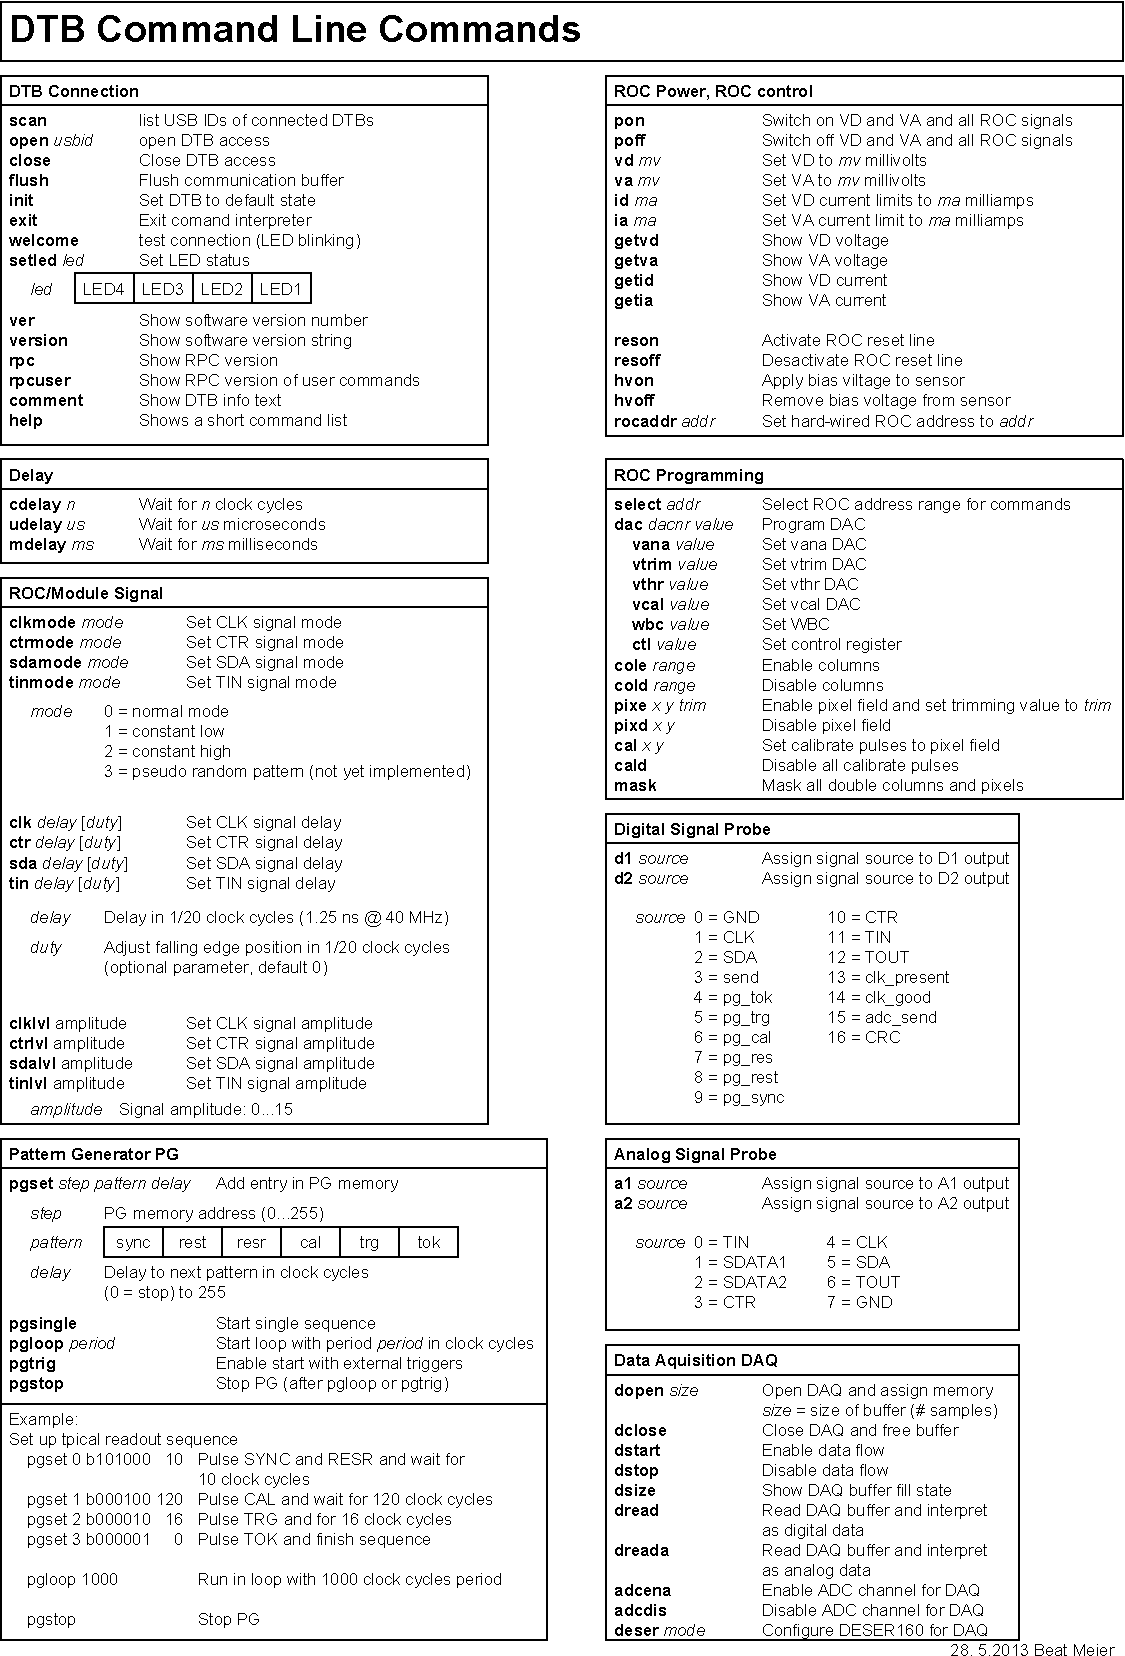
\includegraphics[width=.85\textwidth]{DTB_commands.pdf}

%{\footnotesize
%\begin{tabular}{p{.14\textwidth}p{.35\textwidth}}
%\toprule
%\multicolumn{2}{l}{\textbf{DTB connection}} \\
%scan    & list USB IDs of connected DTBs \\
%open \psiparam{usbid}   & open DTB access to testboard with id \psiparam{usbid} \\
%close   & Close DTB access \\
%flush   & Flush communication buffer \\
%init    & Set DTB to default state \\
%exit    & Exit comand interpreter \\
%welcome & test connection (LED blinking) \\
%setled \psiparam{ledptrn}  & Set LED status. \psiparam{ledptrn} is a 4-bit binary value setting the LED status. Bit 0 sets LED 1 etc. \\
%ver     & Show software version number \\
%version & Show software version string \\
%rpc     & Show RPC version \\
%rpcuser & Show RPC version of user commands \\
%comment & Show DTB info text \\
%help    & Shows a short command list \\
%\midrule
%\multicolumn{2}{l}{\textbf{Execution delay}} \\
%cdelay \psiparam{n}  & Wait for \psiparam{n} clock cycles \\
%udelay \psiparam{us} & Wait for \psiparam{us} microseconds \\
%mdelay \psiparam{ms} & Wait for \psiparam{ms} milliseconds. Note: This command is handled by the computer, not the testboard. \\
%\bottomrule
%\end{tabular}
%}

